\documentclass[doublecol]{../macros/epl2} 
% or \documentclass[page-classic]{epl2} for one column style

\title{Measurement of proton-proton elastic scattering and total cross-section at $\sqrt s = 7\,\rm TeV$}
\shorttitle{Measurement of $\rm pp$ elastic scattering and total cross-section at $\sqrt s = 7\,\rm TeV$} %Insert here a short version of the title if it exceeds 70 characters

\author{
The TOTEM Collaboration -- !! PRELIMINARY !!\\
\iffalse
G.~Antchev\thanks{INRNE-BAS, Institute for Nuclear Research and Nuclear Energy, Bulgarian Academy of Sciences, Sofia, Bulgaria.}\addtocounter{footnote}{-1}
%\addtocounter{footnote}
\and P.~Aspell\inst{8}
\and I.~Atanassov\inst{8}\hspace{-0.15cm}\footnotemark
\and V.~Avati\inst{8}
\and J.~Baechler\inst{8}
\and V.~Berardi\inst{5b,5a}
\and M.~Berretti\inst{7b}
\and E.~Bossini\inst{7b}
\and M.~Bozzo\inst{6b,6a}
\and P.~Brogi\inst{7b}
\and E.~Br\"{u}cken\inst{3a,3b}
\and A.~Buzzo\inst{6a}
\and F.~S.~Cafagna\inst{5a}
\and M.~Calicchio\inst{5b,5a}
\and M.~G.~Catanesi\inst{5a}
\and C.~Covault\inst{9}
\and M.~Csan\'{a}d\inst{4}
\and T.~Cs\"{o}rg\H{o}\inst{4}
\and M.~Deile\inst{8}
 \and K.~Eggert\inst{9}
 \and V.~Eremin\thanks{Ioffe Physical - Technical Institute of Russian Academy of Sciences.}
 \and R.~Ferretti\inst{6a,6b}
 \and F.~Ferro\inst{6a}
 \and A. Fiergolski\thanks{Warsaw University of Technology, Poland.}
 \and F.~Garcia\inst{3a}
 \and S.~Giani\inst{8}
 \and V.~Greco\inst{7b,8}
 \and L.~Grzanka\inst{8}\hspace{-0.15cm}\thanks{Institute of Nuclear Physics, Polish Academy of Science, Cracow, Poland.}\addtocounter{footnote}{-2}
 \and J.~Heino\inst{3a}
 \and T.~Hilden\inst{3a,3b}
 \and M.~R.~Intonti\inst{5a}
%\and M.~Janda\inst{1b}
 \and J.~Ka\v{s}par\inst{1a,8}
 \and J.~Kopal\inst{1a,8}
 \and V.~Kundr\'{a}t\inst{1a}
 \and K.~Kurvinen\inst{3a}
 \and S.~Lami\inst{7a}
 \and G.~Latino\inst{7b}
 \and R.~Lauhakangas\inst{3a}
 \and  T.~Leszko\footnotemark
 %\thanks{Warsaw University of Technology, Poland}
 \and E.~Lippmaa\inst{2}
 \and M.~Lokaj\'{\i}\v{c}ek\inst{1a}
 \and M.~Lo~Vetere\inst{6b,6a}
 \and F.~Lucas~Rodr\'{i}guez\inst{8}
 \and M.~Macr\'{\i}\inst{6a}
 \and L.~Magaletti\inst{5b,5a}
%\and G.~Magazz\`{u}\inst{7a}
 \and T.~M\"aki\inst{3a}
 \and A.~Mercadante\inst{5b,5a}
%\and M.~Meucci\inst7b
 \and N.~Minafra\inst{8} 
 \and S.~Minutoli\inst{6a}\addtocounter{footnote}{1}
 \and F.~Nemes\inst{4}\hspace{-0.15cm}\thanks{Department of Atomic Physics, ELTE University, Hungary.}
 \and H.~Niewiadomski\inst{8}
%\and E.~Noschis\inst{8}
%\and T.~Nov\'{a}k\inst{4}\thanks{KRF,  Gy\"{o}ngy\"{o}s, Hungary}
 \and E.~Oliveri\inst{7b}
 \and F.~Oljemark\inst{3a,3b}
 \and R.~Orava\inst{3a,3b}
 \and M.~Oriunno\inst{8}\hspace{-0.15cm}\thanks{SLAC National Accelerator Laboratory, Stanford CA, USA.}
 \and K.~\"{O}sterberg\inst{3a,3b}
 \and P.~Palazzi\inst{7b}
 \and J.~Proch\'{a}zka\inst{1a}
 \and M.~Quinto\inst{5a}
 \and E.~Radermacher\inst{8}
 \and E.~Radicioni\inst{5a}
 \and F.~Ravotti\inst{8}
 \and E.~Robutti\inst{6a}
 \and L.~Ropelewski\inst{8}
 \and G.~Ruggiero\inst{8}
 \and H.~Saarikko\inst{3a,3b}
% \and G.~Sanguinetti\inst{7a}
 \and A.~Santroni\inst{6b,6a}
 \and A.~Scribano\inst{7b}
 \and W.~Snoeys\inst{8}
 \and J.~Sziklai\inst{4}
 \and C.~Taylor\inst{9}
 \and N.~Turini\inst{7b}
 \and V.~Vacek\inst{1b}
 \and M.~Vitek\inst{1b}
 \and J.~Welti\inst{3a,3b}
 \and J.~Whitmore\inst{10}
\fi
\vskip5cm
 }          %ends author list
\shortauthor{The TOTEM Collaboration (G.~Antchev \etal)}

\institute{
\inst{1a}{Institute of Physics of the Academy of Sciences of the Czech Republic, Praha, Czech Republic.}\\
\inst{1b}{Czech Technical University, Praha, Czech Republic.}\\
\inst{2} {National Institute of Chemical Physics and Biophysics NICPB, Tallinn, Estonia.}\\
\inst{3a}{Helsinki Institute of Physics, Finland.}\\
\inst{3b}{Department of Physics, University of Helsinki, Finland.}\\
\inst{4} {MTA Wigner Research Center, RMKI, Budapest, Hungary.}\\
\inst{5a}{INFN Sezione di Bari, Italy.}\\
\inst{5b}{Dipartimento Interateneo di Fisica di Bari, Italy.}\\
\inst{6a}{Sezione INFN, Genova, Italy.}\\
\inst{6b}{Universit\`{a} degli Studi di Genova, Italy.}\\
\inst{7a}{INFN Sezione di Pisa, Italy.}\\
\inst{7b}{Universit\`{a} degli Studi di Siena and Gruppo Collegato INFN di Siena, Italy.}\\
\inst{8} {CERN, Geneva, Switzerland.}\\
\inst{9} {Case Western Reserve University, Dept. of Physics, Cleveland, OH, USA.}\\
\inst{10}{Penn State University, Dept. of Physics, University Park, PA, USA.}\\
}


\pacs{13.60.Hb}{Total and inclusive cross-sections (including deep-inelastic processes)}


\abstract{%
At the LHC energy of $\sqrt s = 7\un{TeV}$, under various beam and background conditions, luminosities, and Roman Pot positions, TOTEM has measured the differential cross-section for proton-proton elastic scattering as a function of the four-momentum transfer squared $t$. The results of the different analyses are in excellent agreement demonstrating no sizeable dependence on the beam conditions. Due to the very close approach of the Roman Pot detectors to the beam center ($\approx 5\sigma_{\rm beam}$) in a dedicated run with $\beta^*=90\un{m}$, $|t|$-values down to $5\cdot10^{-3}\un{GeV^2}$ were reached. The exponential slope of the differential elastic cross-section in this newly explored $|t|$-region stayed unchanged and hence an exponential fit with only one constant $B = (19.9 \pm 0.3)\un{GeV^{-2}}$ over the large $|t|$-range from $0.005$ to $0.2\un{GeV^2}$ describes well the differential distribution. The high precision of the measurement and the large lever arm lead to an error on the slope parameter $B$ which is remarkably small compared to previous experiments. It allows a precise extrapolation over the non-visible cross-section (only  $9\%$) to $t=0$. With the luminosity from CMS, the elastic cross-section was determined to be $(25.4 \pm 1.1)\un{mb}$, and using in addition the optical theorem, the total $\rm pp$ cross-section was derived to be $(98.6 \pm 2.2)\un{mb}$.
%
For model comparisons the $t$-distributions are tabulated including the large $|t|$-range of the previous measurement \cite{epl95}.
}


\def\d{{\rm d}}
\def\un#1{\,{\rm #1}}
\def\ung#1{\quad[{\rm #1}]}
\def\unt#1{[{\rm #1}]}
\def\e{{\rm e}}

\setbox123\hbox{\small$0$}
\def\S{\hbox to\wd123{\hss}}
\setbox124\hbox{\small$_{0}$}
\def\s{\hbox to\wd124{\hss}}


\begin{document}

\maketitle

%--------------------------------------------------
\section{Introduction}

The study of elastic proton-proton scattering reveals many aspects about the structure of the proton, its shape and opacity, i.e.~matter density. It also tests the interplay of non-perturbative and perturbative $\rm pp$ interactions depending on the four-momentum transfer squared $t$ involved in the scattering process.
% ($t = (p_{\rm i} - p_{\rm f})^2$ with $p_{\rm i,f}$  being the initial and final four-momentum, respectively). 

In several runs with different beam optics, TOTEM has measured at the center-of-mass energy of $7\un{TeV}$ the differential elastic cross-section $\d\sigma/\d t$ over a wide range of $t$. The first measurement, reported by the TOTEM collaboration \cite{epl95}, extended over the $|t|$-range from $0.36 \hbox{ to } 2.5\un{GeV^2}$. These data were taken with the standard 2010 LHC beam optics (with the betatron value at the intersection point $\beta^*$ of $3.5\un{m}$). The differential cross-section $\d\sigma/\d t$ exhibited an exponential decay at low $|t|$ followed by a significant diffractive minimum and at larger $|t|$-values a behavior compatible with the power law already observed at lower energies (see references 1 to 11 in \cite{epl95}).

To access smaller $|t|$-values (at $\sqrt s = 7\un{TeV}$ $|t| = 0.01\un{GeV^2}$ corresponds to a scattering angle of $\approx 29\un{\mu rad}$) the colliding beams must have a beam divergence of a few micro-radians. This can be obtained by either reducing the beam emittance $\epsilon$ or by increasing the betatron value $\beta^*$ (beam divergence $=\sqrt{\epsilon/\beta^*}$). With a dedicated beam optics configuration ($\beta^* = 90\un{m}$) in a special run, TOTEM extended the measurement to $|t|$-values as low as $2\cdot10^{-2}\un{GeV^2}$ \cite{epl96}. This made the extrapolation of the differential cross-section to the optical point at $t=0$ possible and enabled, for the first time at the LHC, the determination of the elastic scattering cross-section as well as the total cross-section via the optical theorem.

In this paper, we concentrate on an improved $t$-distribution measurement with higher statistics and reaching even smaller $|t|$-values using different data sets taken in October 2011, with several special runs at $\beta^* = 90\un{m}$. This time, the detectors, housed in Roman Pots (RP), were put aggressively close to the beam center: $4.8 \hbox{ to } 6.5$ times the transverse beam size $\sigma_{\rm beam}$. This was possible since in this run the beams were scraped by the LHC collimators at a distance of $4\,\sigma_{\rm beam}$ for RP alignment purposes. For the definition of their position, each Roman Pot had to touch this sharp beam edge. After retraction by $0.5$ to $2\,\sigma_{\rm beam}$, TOTEM took data in very clean conditions with only a few colliding bunch pairs and reached $|t|$ values down to $5\cdot10^{-3}\un{GeV^2}$, enabling the observation of $91\%$ of the elastic cross-section -- compared to only $67\%$ previously \cite{epl96}. By extrapolating the differential elastic cross-section to the optical point $t=0$ and using the optical theorem, the total and inelastic cross-sections were also derived. The differential cross-section over the complete $t$-range combining all available measurements with its statistical and systematic uncertainties is tabulated in this article.

\vskip4cm

In a second paper in the same journal issue \cite{P2}, the inelastic cross-section is measured directly, based on triggers from the forward inelastic detectors. This is compared to the inelastic cross-section obtained from elastic scattering via the optical theorem, yielding a cross-section estimate for single diffraction at masses below $3\un{GeV}$ that escape our detection.

A third paper \cite{P3} summarizes the cross-sections obtained with different approaches, including the luminosity independent method. Since the $\rho$ parameter (the ratio of the real to imaginary part of the hadronic scattering amplitude at $t=0$) does not enter in the method of the 2nd paper \cite{P2}, $\rho$ can be determined by comparing the results from the different methods. Furthermore, the luminosity of the LHC was extracted, confirming the more detector-dependent estimates by CMS. 



%--------------------------------------------------
\section{The proton detectors}

The configuration of the TOTEM Roman Pot system and the silicon detector properties have already been described in detail \cite{jinst,epl95,epl96}. For the understanding of the analysis, a few basic  system  properties are repeated. 

The silicon sensors are placed in movable beam-pipe insertions -- Roman Pots -- located symmetrically on either side of the LHC interaction point (IP) 5 at distances of $215$ -- $220\un{m}$ from the IP.

Each RP station is composed of two units (near and far) separated by a distance of about $5\un{m}$. A unit consists of 3 RPs, two approaching the outgoing beam vertically from the top and the bottom and one horizontally. Each RP is equipped with a stack of 10 silicon strip detectors measuring the proton distance to the beam center in both coordinates perpendicular to the beam with a precision of about $11\un{\mu m}$.
%The RPs are moved from the garage position towards the beam center with a precision of $20\un{\mu m}$.
The movement and the alignment of all pots are monitored with a precision better than $20\un{\mu m}$ based on track reconstruction and external alignment tools.

The large lever arm between the near and the far units allows the determination of the scattering angle in both projections with a precision of about $5\un{\mu rad}$. The knowledge of both the track positions and angles is vital in the analysis. 



%--------------------------------------------------
\section{LHC Optics}

The measurement presented in this paper was performed with the $\beta^*=90\un{m}$ optics, which has been described in detail \cite{epl96}; here we repeat only the most important properties. An elastically scattered proton created at the vertex $(x^*, y^*, z^*=0)$ with the horizontal and vertical scattering angles $(\theta_x^*, \theta_y^*)$ is transported through the LHC magnet lattice and hits the Roman Pots at points $(x, y)$:
\begin{equation}
\label{eq:transport}
\begin{array}{rcl}
x = L_x\,\theta^*_x + v_x\,x^*\ &,\quad& y = L_y\,\theta^*_y + v_y\,y^* \\
L_x = 2.9\un{m} \hbox{ (near)}&,\quad& L_y = 240\un{m} \hbox{ (near)}\\
L_x \approx 0\un{m} \hbox{ (far)}&,\quad& L_y = 260\un{m}\hbox{ (far)}\\
\end{array}
\end{equation}
Since $L_x \approx 0$ in the far RP, the corresponding horizontal hit position $x^{\rm F}$ can be used for vertex $x^*$ determination:
\begin{equation}
\label{eq:vertex reconstruction}
x^* = {x^{\rm F}\over v_x}\ .
\end{equation}
The optimal scattering-angle reconstruction formulae differ for the two projections: the vertical angle $\theta^*_y$ is reconstructed from the hit position $y$ (since $v_y\approx 0$) while the horizontal angle $\theta^*_x$ from the track angle $\theta_x$ at the RP:
\begin{equation}
\label{eq:theta reconstruction}
\theta^*_y = {y\over L_y}\ ,\quad
\theta^*_x = {1\over {\d L_x\over \d s}} \left( \theta_x - {\d v_x\over \d s} x^* \right)\ ,
\end{equation}
where $s$ denotes the distance from the interaction point.


%--------------------------------------------------
\section{Data taking}

The presented data were recorded in October 2011. For this analysis, only one colliding bunch-pair was used with an average proton population of $6\cdot10^{10}$ protons/bunch producing an instantaneous luminosity of $6\un{mb^{-1}\, s^{-1}}$ and an average inelastic-interaction rate of $0.03$ per bunch crossing.

During the run three data sets were recorded with different RP distances to the beam center corresponding to minimum values of the four-momentum transfer squared between $(4.6$ and $7.3)\cdot10^{-3}\un{GeV^2}$. The different data sets enabled us to reduce certain systematic uncertainties (alignment, inefficiency corrections, etc.). A run summary is given in Tab.~\ref{tab:datasets}.

The 1st-level trigger benefits from the 20 possible hits (10 planes in both near and far RP) per proton track and is based on a track segment in the near or the far unit. This redundancy guarantees a high trigger efficiency (over $99\%$ per proton). A coincidence between a proton on the left and the right side of the IP is requested in the typical elastic double-arm signature in the vertical RP detectors with two diagonals (left top -- right bottom or left bottom -- right top). The characteristic of the $\beta^* = 90\un{m}$ optics forces most of the elastically scattered protons into the vertical RPs, see Fig.~\ref{fig:hit dist}.

\begin{table}
\caption{Description of the three datasets available. The RP position gives the RP approach to beam in multiples of the beam size ($\sigma_{\rm beam}$). The third column summarizes the numbers of elastic events reconstructed from both diagonals. $\mathcal{L}_{\rm int}$ is the integrated
luminosity for each dataset, taking into account the DAQ inefficiency. The last column shows the lowest $|t|$ values reached.}
\label{tab:datasets}
\begin{center}
\vskip-3mm
\begin{tabular}{ccccc}\hline
& RP & elastic                   & $\mathcal{L}_{\rm int}$ & $|t|_{\rm min}$     \cr
\omit\hss\vbox to 0pt{\vss\hbox{\ dataset\ }\vss}\hss &\multispan4 \cr
 &  position &  events                   & $\unt{\mu b^{-1}}$         & $\unt{GeV^2}$       \cr\hline
1 & $6.5\,\sigma_{\rm beam}$ & 841k      & $68.2$                  & $7.3\cdot10^{-3}$ \cr
2 & $5.5\,\sigma_{\rm beam}$ & 106k      & $8.2$                   & $5.7\cdot10^{-3}$ \cr
3 & $4.8\,\sigma_{\rm beam}$ & 89k       & $6.6$                   & $4.6\cdot10^{-3}$ \cr\hline
\end{tabular}
\end{center}
\end{table}


%--------------------------------------------------
\section{Analysis}

The analysis is very similar to the previous one \cite{epl96}. Here, we take advantage of having three datasets (each with two diagonals) analyzed separately, thus leading to a better control over the systematics.


%-------------------------
\subsection{Alignment}

Three complementary methods were applied \cite{jan_thesis}. First, the RP position was roughly determined from the beam-based alignment \cite{mario_ipac_2011}. Second, proton tracks passing through the overlap between vertical and horizontal RPs were used to determine the relative alignment among the RPs of each unit. Third, since the elastic event tagging does not require precise alignment, an alignment fine-tuning was performed on a sample obtained from an elastic pre-selection. By exploiting the azimuthal symmetry of elastic scattering%
%and taking advantage of the very small effective length $L_x$
, the horizontal and vertical shifts and the tilt of each unit could be adjusted. The effect of residual misalignments on $\d\sigma_{\rm el}/\d t$ was thus smaller than $0.3\%$ for every $t$-bin.


%-------------------------
\subsection{Elastic tagging}

The cuts used to select the elastic events are summarized in Tab.~\ref{tab:cuts}. Cuts 1 and 2 require the reconstructed-track collinearity between the left and right arm. Cuts 3 to 6 effectively work as low-$\xi$ cuts ($\xi$ being the fractional momentum loss of a proton).
Cuts 3 and 4: if $\xi\neq 0$, the vertex reconstruction Eq.~(\ref{eq:vertex reconstruction}) becomes invalid.
Cuts 5 and 6: if $\xi\neq 0$, the correlation between the track position ($y^{\rm N}$) and the track angle (proportional to $y^{\rm F} - y^{\rm N}$) is lost. Cut 7 compares the horizontal vertex position reconstructed from the left and right arms. It is the strongest single cut and is very effective against the beam-halo background, see Fig.~\ref{fig:hit dist}.

\begin{table}
\caption{The elastic selection cuts. The superscripts R and L refer to the right and left arm, the N and F corresponds to the near and far units. The constant $\alpha = L_y^{\rm F} / L_y^{\rm N} - 1 \approx 0.11$. The right-most column gives the RMS of the cut distribution ($\equiv 1\sigma$), all cuts are applied at $3\sigma$-level.
}
\label{tab:cuts}
\begin{center}
\begin{tabular}{ccc}\hline
number & cut & RMS\cr\hline
diagonal &\multispan2 \hss track reconstructed in all 4 diagonal RPs \hss \cr
1 & $\theta_x^{*\rm R} - \theta_x^{*\rm L}$		& $9.2\un{\mu rad}$	\cr
2 & $\theta_y^{*\rm R} - \theta_y^{*\rm L}$		& $3.5\un{\mu rad}$	\cr
3 & $|x^{*\rm R}|$ 									& $200\un{\mu m}$	\cr
4 & $|x^{*\rm L}|$ 									& $200\un{\mu m}$	\cr
5 & $\alpha\,y^{\rm R,N} - (y^{\rm R,F} - y^{\rm R,N})$	& $17\un{\mu m}$	\cr
6 & $\alpha\,y^{\rm L,N} - (y^{\rm L,F} - y^{\rm L,N})$	& $17\un{\mu m}$	\cr
7 & $x^{*\rm R} - x^{*\rm L}$					& $9\un{\mu m}$ 	\cr\hline
\end{tabular}
\end{center}
\end{table}


%-------------------------
\subsection{Kinematics reconstruction}

The scattering angles were reconstructed for each arm according to Eq.~(\ref{eq:theta reconstruction}). The corresponding uncertainties were $1.3\%$ and $0.8\%$ for $\theta^*_x$ and $\theta^*_y$, respectively. The former has a more pronounced effect on $\d\sigma_{\rm el}/\d t$
%(due to its higher value and the absence of limitations like the $\theta^*_y$ aperture limitation shown in Fig.~\ref{fig:hit dist})
and is the leading systematic uncertainty for larger $|t|$ values, cf.~Tab.~\ref{tab:systematics}.

For elastic events, the angles reconstructed from left and right arms were averaged, which leads to an uncertainty reduction.

%-------------------------
\subsection{Background}

The background contribution (i.e.~all non-elastic events passing the selection cuts) was estimated by omitting the strongest single cut (number 7 in Tab.~\ref{tab:cuts}) and analyzing the distribution of $x^{*\rm R} - x^{*\rm L}$. This distribution can be reasonably described by two Gaussians -- one for the signal and one for the background. By interpolating the background tails ($|\Delta x^*| > 3\sigma$) into the signal region ($|\Delta x^*| < 3\sigma$), the background/signal ratio was determined as $(0.8 \pm 0.4)\%$.


%-------------------------
\subsection{Acceptance correction}

We identified two acceptance limitations: the detector edge (relevant for low $|t|$) and the LHC aperture limitation shown in Fig.~\ref{fig:hit dist} right (relevant for high $|t|$). Both effects were treated by assuming azimuthal symmetry of the elastic scattering and by correcting for smearing around the limitation edges. In order to keep the uncertainty on a reasonable level, we constrained ourselves to the region where the full acceptance correction was not larger than a factor $7.5$%
%(considering both diagonals)
.


%-------------------------
\subsection{Unfolding of resolution effects}

The angular resolution was determined by comparing the scattering angles reconstructed from the left and right arm. Combining all three datasets and all diagonals yields one-arm resolutions of $(6.36\pm 0.21)\un{\mu rad}$ in $\theta^*_x$ and $(2.47\pm 0.07)\un{\mu rad}$ in $\theta^*_y$. The latter is predominantly given by the beam-divergence, whereas the $\theta^*_x$ resolution is deteriorated by a contribution from the finite detector pitch.

The $t$-resolution impact on $\d\sigma_{\rm el}/\d t$  was determined (and eliminated) by an iterative procedure, that starts by taking the observed (smeared) $t$-distribution as an input to a Monte-Carlo calculation of the un-smearing correction. The correction is applied to the observed $t$-distribution and yields a better estimate of the true $t$-distribution. These two steps were repeated three times to reach convergence. The systematic uncertainty of this procedure (due to the uncertainty of the $\theta^*_{x, y}$ resolution) was estimated to be smaller than $0.5\%$.

%-------------------------
\subsection{Efficiencies}

The efficiency of the RP trigger was estimated using the zero-bias data stream. We repeated the elastic event selection on these data and found the RP trigger efficient for all the selected events. Therefore, at $68\%$ confidence level, we concluded the trigger efficiency to be higher than $99.8\%$.
% 95% CL: 99.40

The DAQ inefficiency (dead time) was determined by comparing the numbers of triggered and recorded events, yielding $(1.858 \pm 0.001)\%$.

There are several reasons for reconstruction inefficiency: intrinsic RP detection inefficiency of each silicon sensor, proton interactions with the material of a RP and ``pile-up'' of several protons in one event (RPs can uniquely reconstruct only one track). For the last case, the most important contribution is a coincidence of an elastic proton and a beam-halo proton, see Fig.~\ref{fig:hit dist}.

Uncorrelated inefficiencies of single RPs were studied by removing the examined RP from the selection cuts and counting the recuperated events. For this study, only cut 2 could be kept -- the others require both near and far RP measurements. The result was an inefficiency of $(1.5 \pm 0.2)\%$ for the near and $(3.0 \pm 0.2)\%$ for the far RPs. This difference can be explained by proton interactions in the near RP that affect the far RP too. This near-far correlated inefficiency was determined from data by counting events with corresponding shower signatures, yielding $(1.5\pm 0.7)\%$ (this result is confirmed by MC simulations).

The ``pile-up'' inefficiency was calculated from the probability of finding an additional track (on top of the elastic) in any station of a diagonal. This probability was determined from the zero-bias data stream and was found to increase as th RPs approached the beam. For instance, for the diagonal bottom-left top-right, the probabilities were $(3.9 \pm 0.3)\%$, $(6.2 \pm 0.3)\%$ and $(7.9 \pm 0.3)\%$ for the datasets 1, 2 and 3, respectively.


\begin{figure*}
\hbox{}\vskip-7mm
\begin{center}
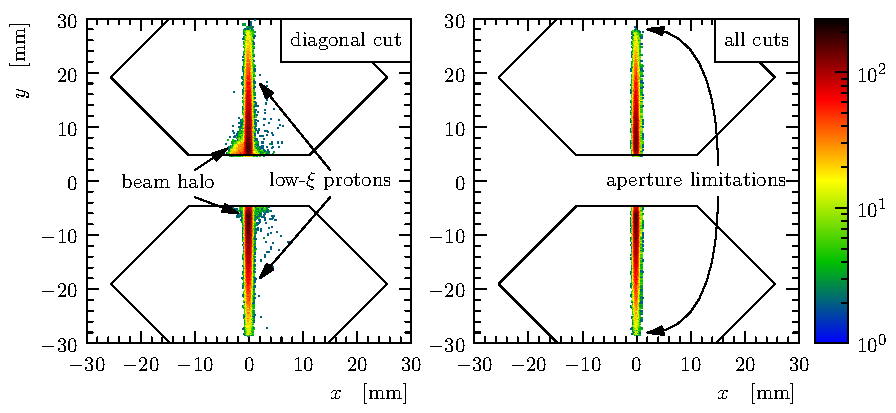
\includegraphics{fig/hit_dist.pdf}
\vskip-5mm
\caption{Hit distributions from dataset 3 in the far unit of the $220\un{m}$ station, right arm. Left: with diagonal cut only, Right: with all the elastic selection cuts (see Tab.~\ref{tab:cuts}). The left plot clearly indicates the presence of the beam halo, which is eliminated by the selection cuts (the right plot). The distribution of elastic hits in the right plot is sharply cut at about $|y| = 29\un{mm}$ as a consequence of the LHC aperture limitations. }
\label{fig:hit dist}
\end{center}
\end{figure*}

%-------------------------
\subsection{Luminosity}

In this paper, we use the luminosity measured by CMS with a $4\%$-uncertainty estimate%
%(no dedicated low-luminosity performance studies have been performed)
. Luminosity-independent results are given elsewhere \cite{P3}.

% Ken's pedestal subtraction

\subsection{Extrapolation to $t=0$}

The elastic differential cross-section was extrapolated to zero with the following parameterization:
\begin{equation}
\label{eq:extrapolation}
{\d\sigma_{\rm el}\over \d t} = \left. {\d\sigma_{\rm el}\over \d t}\right|_{t=0} \ \e^{-B|t|}\ .
\end{equation}
The fits were performed from the lowest accessible $|t|$ values (see $|t|_{\rm min}$ in Tab.~\ref{tab:datasets}) to $|t| = 0.2\un{GeV^2}$, with a typical $\chi^2/\hbox{n.d.f.}$ of $1.2$ -- see for example the black line in Fig.~\ref{fig:dsdt}.

%-------------------------
\section{Systematic uncertainty calculation}

% Statistical uncertainty negligible, see Tab.~\ref{tab:results}.

For each of the analysis steps above, the systematic uncertainty effect on $\d\sigma_{\rm el}/\d t$ was estimated with a Monte-Carlo simulation. Tab.~\ref{tab:systematics} summarizes these uncertainties for several $|t|$ values, grouping the contributions into three categories: $t$-dependent, $t$-independent (normalization) and luminosity uncertainties. Since there are a number of contributions in each category, the uncertainties were combined in quadrature.

The luminosity uncertainty is the leading systematic effect for $|t| < 0.2\un{GeV^2}$, above that point it is the uncertainty of $\d L_x/\d s$. The optics-related error contribution is almost vanishing around $|t| = 0.06\un{GeV^2}$ and has opposite signs below and above that point. Therefore there is a partial error cancellation in the integrated elastic cross-section $\sigma_{\rm el}$, and consequently the relative error of $\sigma_{\rm el}$ is significantly lower than the one of $\d\sigma_{\rm el}/\d t|_0$ -- see Tab.~\ref{tab:results}. Moreover, there is a strong correlation between the errors of $\sigma_{\rm el}$ and $\d\sigma_{\rm el}/\d t|_0$ -- the correlation coefficient is $0.76$.
% (when both $t$-dependent and normalization contributions are included).


\begin{table*}
\hbox{}\vskip-14mm
\begin{minipage}{9.4cm}
\caption{Overview of the systematic uncertainties of the differential cross-section $\d\sigma_{\rm el}/\d t$.}
\vskip-3mm
\label{tab:systematics}
\begin{center}
\small
\setlength{\tabcolsep}{5.0pt}
\begin{tabular}{cccccccccc}\hline
\iffalse
$|t|\ung{GeV^2}$ &	0.005 &	0.01 &	0.06 &	0.1 &	0.12 &	0.16 &	0.2 &	0.3 &	0.4\cr\hline
$t$-dependent &	1.8\% &	1.0\% &	0.3\% &	0.9\% &	1.2\% &	3.0\% &	4.4\% &	8.3\% &	12.3\%\cr
normalization &\multispan9\hfil	1.2\%\hfil  \cr
luminosity &\multispan9\hfil	4.0\%\hfil  \cr\hline
total &	4.5\% &	4.3\% &	4.2\% &	4.3\% &	4.3\% &	5.1\% &	6.1\% &	9.3\% &	12.9\% \cr\hline
\fi
$|t|\ung{GeV^2}$ & $t$-dependent & normalization & luminosity & total\cr
\hline
$0.005$	&	$1.8\%$		& $\cdot$	& $\cdot$ 	& $4.5\%$ \cr
$0.01$	&	$1.0\%$		& $\cdot$	& $\cdot$ 	& $4.3\%$ \cr
$0.06$	&	$0.3\%$		& $\cdot$	& $\cdot$ 	& $4.2\%$ \cr
$0.1$	&	$0.9\%$		& $\cdot$	& $\cdot$ 	& $4.3\%$ \cr
$0.12$	&	$1.2\%$		& $1.2\%$	& $4.0\%$	& $4.3\%$ \cr
$0.16$	&	$3.0\%$		& $\cdot$	& $\cdot$ 	& $5.1\%$ \cr
$0.2$	&	$4.4\%$		& $\cdot$	& $\cdot$ 	& $6.1\%$ \cr
$0.3$	&	$8.3\%$		& $\cdot$	& $\cdot$ 	& $9.3\%$ \cr
$0.4$	&	$12.3\%$	& $\cdot$	& $\cdot$ 	& $12.9\%$ \cr
\hline
\end{tabular}
\end{center}
\end{minipage}
%
\hfill
%
% the commands below ensure that the following minipage is treated as figure, although it is in table environment
\catcode`\@=11
\def\@captype{figure}%
%
\begin{minipage}{7.7cm}
\begin{center}
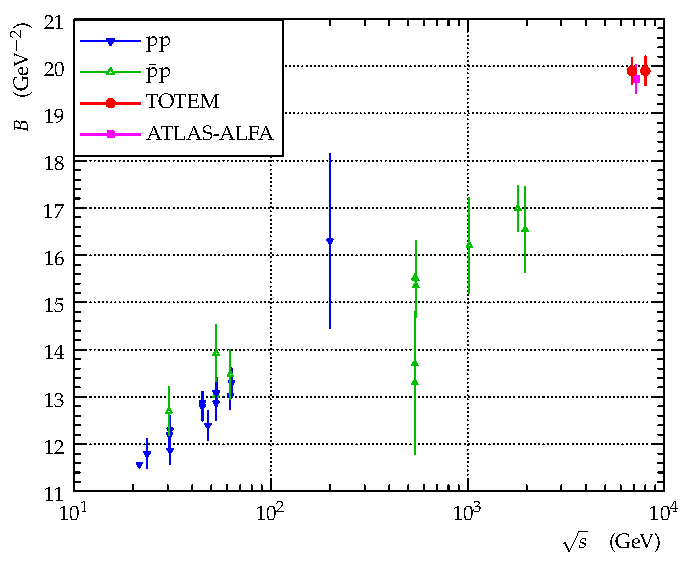
\includegraphics{fig/B_s.pdf}
\vskip-5mm
\caption{The elastic slope $B$ (see Eq.~(\ref{eq:extrapolation})) as a function of the scattering energy $\sqrt s$.
%$\rm pp$ and $\rm \bar pp$ data from \cite{pdg}.
}
\label{fig:B s}
\end{center}
\end{minipage}
%
\end{table*}



\begin{figure*}
\hbox{}\vskip-8mm
\begin{center}
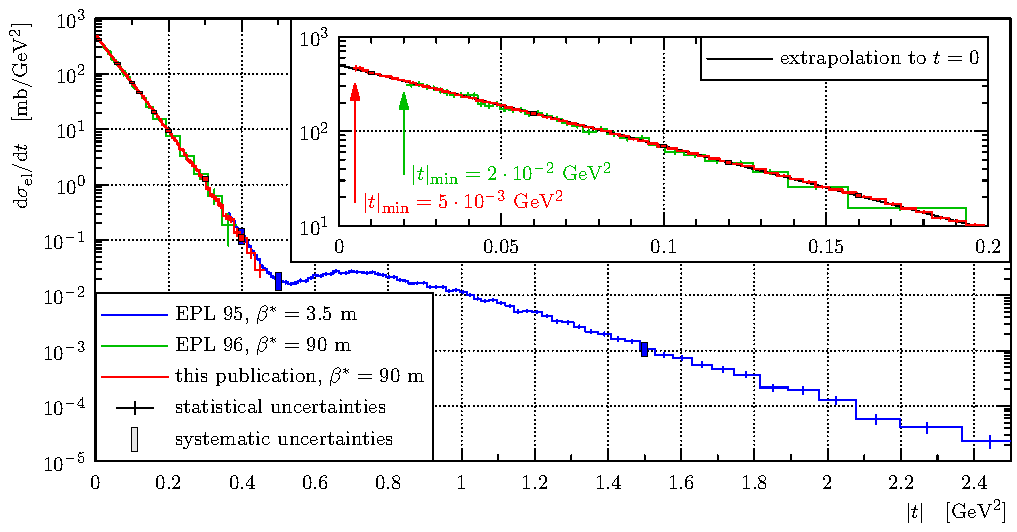
\includegraphics{fig/dsdt_comp.pdf}
\vskip-5mm
\caption{A compilation of the elastic differential cross-section measurements by TOTEM. Each measurement is shown in a different color. The embedded figure provides a zoom of the region used for extrapolation to $t=0$, showing the lowest $|t|$-values accessible in the analysis from Ref.~\cite{epl96} (green) and this analysis (red).}
\label{fig:dsdt}
\end{center}
\vskip-15mm\hbox{}
\end{figure*}


\begin{largetable}
\hbox{}\vskip-8.4mm
\caption{The elastic differential cross-section determined in this analysis. Some details on the systematic uncertainty calculation can be found in Tab.~\ref{tab:systematics}, which can also be used to evaluate the correlations of the systematic uncertainties among the bins (the three contributions are independent).
}
\label{tab:data low t}
\begin{center}
%\vskip-3mm
\small
\setlength{\tabcolsep}{3.5pt}
\begin{tabular}{cc@{$\pm$}c@{$\pm$}cccc@{$\pm$}c@{$\pm$}cccc@{$\pm$}c@{$\pm$}cccc@{$\pm$}c@{$\pm$}c}
\multispan4\hrulefill&&\multispan4\hrulefill&&\multispan4\hrulefill&&\multispan4\hrulefill\cr
$|t|$ & \multispan3\hss${\d \sigma_{\rm el}\over\d t} \ung{mb/GeV^2}$\hss&&
$|t|$ & \multispan3\hss${\d \sigma_{\rm el}\over\d t} \ung{mb/GeV^2}$\hss&&
$|t|$ & \multispan3\hss${\d \sigma_{\rm el}\over\d t} \ung{mb/GeV^2}$\hss&&
$|t|$ & \multispan3\hss${\d \sigma_{\rm el}\over\d t} \ung{mb/GeV^2}$\hss
\cr
$\unt{GeV^2}$ &&stat&syst&&
$\unt{GeV^2}$ &&stat&syst&&
$\unt{GeV^2}$ &&stat&syst&&
$\unt{GeV^2}$ &&stat&syst
\cr
\multispan4\hrulefill&&\multispan4\hrulefill&&\multispan4\hrulefill&&\multispan4\hrulefill\cr
$0.00515$ & $465.\S$ & $27.\S$ & $21.\S$ && $0.0477$ & $197.2\S$ & $1.3\S$ & $8.3\S$ && $0.106$ & $61.90$ & $0.58$ & $2.66$ && $0.196$ & $10.11\S$ & $0.23\S$ & $0.61\S$ \cr
$0.00650$ & $465.\S$ & $11.\S$ & $21.\S$ && $0.0499$ & $187.5\S$ & $1.3\S$ & $7.9\S$ && $0.109$ & $58.11$ & $0.55$ & $2.50$ && $0.201$ & $\S9.31\S$ & $0.22\S$ & $0.57\S$ \cr
$0.00818$ & $437.5$ & $\S5.0$ & $19.1$ && $0.0522$ & $178.1\S$ & $1.2\S$ & $7.5\S$ && $0.112$ & $54.11$ & $0.53$ & $2.33$ && $0.207$ & $\S8.07\S$ & $0.21\S$ & $0.51\S$ \cr
$0.00995$ & $411.0$ & $\S3.3$ & $17.7$ && $0.0545$ & $168.8\S$ & $1.2\S$ & $7.1\S$ && $0.116$ & $51.21$ & $0.51$ & $2.20$ && $0.213$ & $\S6.98\S$ & $0.19\S$ & $0.45\S$ \cr
$0.0117\S$ & $402.3$ & $\S2.9$ & $17.3$ && $0.0569$ & $162.5\S$ & $1.1\S$ & $6.8\S$ && $0.119$ & $48.24$ & $0.49$ & $2.07$ && $0.219$ & $\S6.22\S$ & $0.17\S$ & $0.42\S$ \cr
$0.0135\S$ & $384.5$ & $\S2.6$ & $16.5$ && $0.0592$ & $155.5\S$ & $1.1\S$ & $6.5\S$ && $0.122$ & $44.99$ & $0.46$ & $1.96$ && $0.225$ & $\S5.38\S$ & $0.16\S$ & $0.37\S$ \cr
$0.0154\S$ & $378.0$ & $\S2.4$ & $16.2$ && $0.0616$ & $149.4\S$ & $1.1\S$ & $6.3\S$ && $0.126$ & $42.74$ & $0.45$ & $1.89$ && $0.232$ & $\S4.40\S$ & $0.14\S$ & $0.31\S$ \cr
$0.0172\S$ & $360.3$ & $\S2.3$ & $15.4$ && $0.0641$ & $140.2\S$ & $1.0\S$ & $5.9\S$ && $0.130$ & $39.49$ & $0.43$ & $1.77$ && $0.239$ & $\S4.25\S$ & $0.14\S$ & $0.31\S$ \cr
$0.0191\S$ & $348.1$ & $\S2.2$ & $14.9$ && $0.0666$ & $135.10$ & $0.99$ & $5.70$ && $0.133$ & $35.75$ & $0.43$ & $1.63$ && $0.246$ & $\S3.47\S$ & $0.13\S$ & $0.26\S$ \cr
$0.0210\S$ & $337.0$ & $\S2.1$ & $14.4$ && $0.0691$ & $129.00$ & $0.96$ & $5.45$ && $0.137$ & $33.63$ & $0.41$ & $1.56$ && $0.253$ & $\S2.82\S$ & $0.11\S$ & $0.22\S$ \cr
$0.0229\S$ & $325.0$ & $\S2.0$ & $13.9$ && $0.0716$ & $120.53$ & $0.91$ & $5.10$ && $0.141$ & $31.08$ & $0.41$ & $1.47$ && $0.261$ & $\S2.52\S$ & $0.10\S$ & $0.20\S$ \cr
$0.0248\S$ & $307.9$ & $\S1.9$ & $13.1$ && $0.0742$ & $115.10$ & $0.89$ & $4.88$ && $0.145$ & $28.91$ & $0.39$ & $1.39$ && $0.270$ & $\S2.142$ & $0.097$ & $0.178$ \cr
$0.0268\S$ & $296.7$ & $\S1.8$ & $12.7$ && $0.0769$ & $109.63$ & $0.86$ & $4.65$ && $0.149$ & $25.65$ & $0.38$ & $1.25$ && $0.278$ & $\S1.824$ & $0.086$ & $0.157$ \cr
$0.0287\S$ & $285.9$ & $\S1.8$ & $12.2$ && $0.0795$ & $104.97$ & $0.83$ & $4.46$ && $0.153$ & $24.16$ & $0.36$ & $1.20$ && $0.287$ & $\S1.455$ & $0.075$ & $0.129$ \cr
$0.0307\S$ & $275.3$ & $\S1.7$ & $11.7$ && $0.0823$ & $100.22$ & $0.80$ & $4.27$ && $0.157$ & $22.35$ & $0.35$ & $1.13$ && $0.297$ & $\S1.257$ & $0.069$ & $0.116$ \cr
$0.0328\S$ & $263.0$ & $\S1.6$ & $11.2$ && $0.0850$ & $\S93.18$ & $0.76$ & $3.97$ && $0.162$ & $20.22$ & $0.34$ & $1.04$ && $0.307$ & $\S0.848$ & $0.055$ & $0.081$ \cr
$0.0348\S$ & $252.0$ & $\S1.6$ & $10.7$ && $0.0878$ & $\S89.16$ & $0.74$ & $3.81$ && $0.166$ & $19.01$ & $0.32$ & $1.00$ && $0.318$ & $\S0.633$ & $0.046$ & $0.063$ \cr
$0.0369\S$ & $242.8$ & $\S1.5$ & $10.3$ && $0.0907$ & $\S81.78$ & $0.70$ & $3.50$ && $0.171$ & $16.92$ & $0.30$ & $0.91$ && $0.330$ & $\S0.558$ & $0.043$ & $0.058$ \cr
$0.0390\S$ & $231.6$ & $\S1.5$ & $\S9.8$ && $0.0936$ & $\S78.85$ & $0.68$ & $3.38$ && $0.175$ & $15.20$ & $0.29$ & $0.83$ && $0.342$ & $\S0.417$ & $0.038$ & $0.045$ \cr
$0.0411\S$ & $222.2$ & $\S1.4$ & $\S9.4$ && $0.0966$ & $\S73.92$ & $0.65$ & $3.17$ && $0.180$ & $13.90$ & $0.28$ & $0.78$ && $0.356$ & $\S0.269$ & $0.027$ & $0.030$ \cr
$0.0433\S$ & $210.9$ & $\S1.4$ & $\S8.9$ && $0.0996$ & $\S68.77$ & $0.62$ & $2.96$ && $0.185$ & $12.09$ & $0.26$ & $0.69$ && $0.371$ & $0.235\S$ & $0.025\S$ & $0.028\S$ \cr
\multispan4&&\multispan4&&\multispan4&&\multispan4\hrulefill\cr
$0.0455\S$ & $204.8$ & $\S1.3$ & $\S8.7$ && $0.103\S$ & $\S65.53$ & $0.60$ & $2.82$ && $0.190$ & $11.26$ & $0.25$ & $0.66$ && \cr
\multispan4\hrulefill&&\multispan4\hrulefill&&\multispan4\hrulefill&\cr
\end{tabular}
\end{center}
\end{largetable}


\begin{largetable}
\hbox{}\vskip-8.4mm
\caption{The elastic differential cross-section as given in \cite{epl95}. The systematic errors almost fully correlated among the bins.
%systematic uncertainties evaluated for three $|t|$ values: $^{+25}_{-37}\%$ at $|t|=0.4\un{GeV^2}$, $^{+28}_{-39}\%$ at $0.5\un{GeV^2}$ and $^{+27}_{-30}\%$ at $1.5\un{GeV^2}$.
}
\label{tab:data medium t}
\begin{center}
%\vskip-3mm
\small
\setlength{\tabcolsep}{2.55pt}%
\def\bs{2.5pt}%
\begin{tabular}{c@{$\pm$}cc@{$\pm$}c@{$\pm$}cc@{\hskip\bs}  c@{$\pm$}cc@{$\pm$}c@{$\pm$}cc@{\hskip\bs}  c@{$\pm$}cc@{$\pm$}c@{$\pm$}cc@{\hskip\bs}  c@{$\pm$}cc@{$\pm$}c@{$\pm$}c}
\multispan5\hrulefill&&\multispan5\hrulefill&&\multispan5\hrulefill&&\multispan5\hrulefill\cr
\multispan2\hss $|t|$\hss & \multispan3\hss${\d \sigma_{\rm el}\over \d t}\ {\rm[\mu b/GeV^2]}$\hss&&
\multispan2\hss $|t|$\hss & \multispan3\hss${\d \sigma_{\rm el}\over \d t}\ {\rm[\mu b/GeV^2]}$\hss&&
\multispan2\hss $|t|$\hss & \multispan3\hss${\d \sigma_{\rm el}\over \d t}\ {\rm[\mu b/GeV^2]}$\hss&&
\multispan2\hss $|t|$\hss & \multispan3\hss${\d \sigma_{\rm el}\over \d t}\ {\rm[\mu b/GeV^2]}$\hss
\cr
\multispan2\hss$\unt{GeV^2}$\hss &&stat&syst&&
\multispan2\hss$\unt{GeV^2}$\hss &&stat&syst&&
\multispan2\hss$\unt{GeV^2}$\hss &&stat&syst&&
\multispan2\hss$\unt{GeV^2}$\hss &&stat&syst
\cr
\multispan5\hrulefill&&\multispan5\hrulefill&&\multispan5\hrulefill&&\multispan5\hrulefill\cr
$0.377$ & $0.002$ & $225.\S$ & $6.\S$ & $^{55.\s}_{82.\s}$  &&  $0.574$ & $0.004$ & $18.3$ & $0.9$ & $^{5.1}_{7.0}$  &&  $0.863$ & $0.005$ & $16.3$ & $0.6$ & $^{4.5}_{5.8}$  &&  $1.290$ & $0.009$ & $3.3\S\S$ & $0.2\S\S$ & $^{0.9\s\s}_{1.0\s\s}$ \cr
$0.384$ & $0.002$ & $174.\S$ & $5.\S$ & $^{43.\s}_{64.\s}$  &&  $0.588$ & $0.004$ & $20.8$ & $0.9$ & $^{5.8}_{7.9}$  &&  $0.880$ & $0.005$ & $16.4$ & $0.6$ & $^{4.5}_{5.8}$  &&  $1.322$ & $0.009$ & $2.7\S\S$ & $0.2\S\S$ & $^{0.7\s\s}_{0.9\s\s}$ \cr
$0.391$ & $0.002$ & $157.\S$ & $4.\S$ & $^{39.\s}_{58.\s}$  &&  $0.602$ & $0.004$ & $22.8$ & $1.0$ & $^{6.4}_{8.7}$  &&  $0.897$ & $0.005$ & $16.9$ & $0.6$ & $^{4.7}_{6.0}$  &&  $1.355$ & $0.010$ & $2.2\S\S$ & $0.1\S\S$ & $^{0.6\s\s}_{0.7\s\s}$ \cr
$0.398$ & $0.002$ & $133.\S$ & $4.\S$ & $^{33.\s}_{49.\s}$  &&  $0.616$ & $0.004$ & $22.2$ & $1.0$ & $^{6.2}_{8.4}$  &&  $0.913$ & $0.005$ & $14.1$ & $0.6$ & $^{3.9}_{5.0}$  &&  $1.390$ & $0.011$ & $2.0\S\S$ & $0.1\S\S$ & $^{0.5\s\s}_{0.6\s\s}$ \cr
$0.405$ & $0.002$ & $116.\S$ & $3.\S$ & $^{29.\s}_{43.\s}$  &&  $0.629$ & $0.004$ & $24.2$ & $1.0$ & $^{6.8}_{9.2}$  &&  $0.931$ & $0.005$ & $14.0$ & $0.6$ & $^{3.9}_{4.9}$  &&  $1.428$ & $0.011$ & $1.6\S\S$ & $0.1\S\S$ & $^{0.4\s\s}_{0.5\s\s}$ \cr
$0.412$ & $0.002$ & $\S93.\S$ & $3.\S$ & $^{23.\s}_{34.\s}$  &&  $0.643$ & $0.004$ & $24.7$ & $1.0$ & $^{6.9}_{9.3}$  &&  $0.948$ & $0.005$ & $14.1$ & $0.6$ & $^{3.9}_{4.9}$  &&  $1.467$ & $0.011$ & $1.5\S\S$ & $0.1\S\S$ & $^{0.4\s\s}_{0.4\s\s}$ \cr
$0.420$ & $0.002$ & $\S78.\S$ & $2.\S$ & $^{20.\s}_{29.\s}$  &&  $0.657$ & $0.004$ & $27.4$ & $1.1$ & $^{7.6}_{0.3}$  &&  $0.966$ & $0.005$ & $11.9$ & $0.5$ & $^{3.3}_{4.1}$  &&  $1.507$ & $0.012$ & $1.1\S\S$ & $0.1\S\S$ & $^{0.3\s\s}_{0.3\s\s}$ \cr
$0.428$ & $0.002$ & $\S63.\S$ & $2.\S$ & $^{16.\s}_{24.\s}$  &&  $0.671$ & $0.004$ & $24.8$ & $1.0$ & $^{6.9}_{9.3}$  &&  $0.985$ & $0.006$ & $12.2$ & $0.5$ & $^{3.4}_{4.2}$  &&  $1.552$ & $0.014$ & $0.84\S$ & $0.07\S$ & $^{0.23\s}_{0.25\s}$ \cr
$0.436$ & $0.002$ & $\S54.\S$ & $2.\S$ & $^{14.\s}_{20.\s}$  &&  $0.685$ & $0.004$ & $25.1$ & $1.0$ & $^{7.0}_{9.4}$  &&  $1.005$ & $0.006$ & $11.3$ & $0.5$ & $^{3.1}_{3.9}$  &&  $1.603$ & $0.015$ & $0.75\S$ & $0.07\S$ & $^{0.20\s}_{0.22\s}$ \cr
$0.445$ & $0.003$ & $\S45.\S$ & $1.\S$ & $^{12.\s}_{17.\s}$  &&  $0.700$ & $0.004$ & $27.3$ & $1.0$ & $^{7.6}_{0.2}$  &&  $1.024$ & $0.006$ & $10.0$ & $0.4$ & $^{2.8}_{3.4}$  &&  $1.656$ & $0.016$ & $0.56\S$ & $0.05\S$ & $^{0.15\s}_{0.16\s}$ \cr
$0.454$ & $0.003$ & $\S34.\S$ & $1.\S$ & $^{\s9.\s}_{13.\s}$  &&  $0.714$ & $0.004$ & $26.5$ & $1.0$ & $^{7.4}_{9.8}$  &&  $1.044$ & $0.006$ & $\S8.7$ & $0.4$ & $^{2.4}_{3.0}$  &&  $1.713$ & $0.017$ & $0.46\S$ & $0.05\S$ & $^{0.12\s}_{0.13\s}$ \cr
$0.464$ & $0.003$ & $\S30.\S$ & $1.\S$ & $^{\s8.\s}_{12.\s}$  &&  $0.728$ & $0.004$ & $25.9$ & $1.0$ & $^{7.2}_{9.6}$  &&  $1.065$ & $0.006$ & $\S7.9$ & $0.4$ & $^{2.2}_{2.7}$  &&  $1.777$ & $0.020$ & $0.37\S$ & $0.04\S$ & $^{0.10\s}_{0.10\s}$ \cr
$0.474$ & $0.003$ & $\S26.\S$ & $1.\S$ & $^{\s7.\s}_{10.\s}$  &&  $0.742$ & $0.004$ & $25.0$ & $0.9$ & $^{7.0}_{9.2}$  &&  $1.086$ & $0.006$ & $\S8.1$ & $0.4$ & $^{2.2}_{2.7}$  &&  $1.851$ & $0.023$ & $0.22\S$ & $0.03\S$ & $^{0.06\s}_{0.06\s}$ \cr
$0.485$ & $0.003$ & $\S21.6$ & $0.9$ & $^{\s5.9}_{\s8.4}$  &&  $0.757$ & $0.004$ & $26.0$ & $0.9$ & $^{7.2}_{9.5}$  &&  $1.108$ & $0.006$ & $\S7.2$ & $0.3$ & $^{2.0}_{2.4}$  &&  $1.932$ & $0.024$ & $0.19\S$ & $0.03\S$ & $^{0.05\s}_{0.05\s}$ \cr
$0.496$ & $0.003$ & $\S19.5$ & $0.9$ & $^{\s5.4}_{\s7.6}$  &&  $0.771$ & $0.004$ & $24.1$ & $0.9$ & $^{6.7}_{8.8}$  &&  $1.131$ & $0.007$ & $\S6.5$ & $0.3$ & $^{1.8}_{2.2}$  &&  $2.024$ & $0.029$ & $0.13\S$ & $0.02\S$ & $^{0.03\s}_{0.03\s}$ \cr
$0.508$ & $0.003$ & $\S18.0$ & $0.8$ & $^{\s5.0}_{\s7.0}$  &&  $0.786$ & $0.004$ & $23.2$ & $0.8$ & $^{6.4}_{8.4}$  &&  $1.155$ & $0.007$ & $\S5.1$ & $0.3$ & $^{1.4}_{1.7}$  &&  $2.133$ & $0.034$ & $0.059$ & $0.012$ & $^{0.015}_{0.014}$ \cr
$0.520$ & $0.004$ & $\S17.1$ & $0.8$ & $^{\s4.8}_{\s6.6}$  &&  $0.801$ & $0.004$ & $21.3$ & $0.8$ & $^{5.9}_{7.7}$  &&  $1.179$ & $0.007$ & $\S5.3$ & $0.3$ & $^{1.4}_{1.7}$  &&  $2.272$ & $0.048$ & $0.041$ & $0.008$ & $^{0.011}_{0.010}$ \cr
$0.533$ & $0.004$ & $\S16.1$ & $0.8$ & $^{\s4.5}_{\s6.2}$  &&  $0.816$ & $0.004$ & $21.6$ & $0.8$ & $^{6.0}_{7.8}$  &&  $1.205$ & $0.008$ & $\S5.0$ & $0.3$ & $^{1.4}_{1.6}$  &&  $2.443$ & $0.050$ & $0.023$ & $0.005$ & $^{0.006}_{0.005}$ \cr
\multispan5&&\multispan5&&\multispan5&&\multispan5\hrulefill\cr
$0.547$ & $0.004$ & $\S16.9$ & $0.8$ & $^{\s4.7}_{\s6.5}$  &&  $0.831$ & $0.004$ & $18.9$ & $0.7$ & $^{5.2}_{6.8}$  &&  $1.232$ & $0.008$ & $\S4.2$ & $0.2$ & $^{1.2}_{1.4}$  \cr
$0.560$ & $0.004$ & $\S18.5$ & $0.9$ & $^{\s5.2}_{\s7.1}$  &&  $0.847$ & $0.005$ & $18.3$ & $0.7$ & $^{5.1}_{6.6}$  &&  $1.261$ & $0.008$ & $\S3.4$ & $0.2$ & $^{0.9}_{1.1}$  \cr
\multispan5\hrulefill&&\multispan5\hrulefill&&\multispan5\hrulefill&&\multispan5\cr
\end{tabular}
\end{center}
\end{largetable}



\begin{table*}
\hbox{}\vskip-9.4mm
\caption{Result summary with detailed systematic uncertainty composition. The $t$-dependent, normalization and luminosity uncertainties correspond to those presented in Tab.~\ref{tab:systematics}. The $\rho$ uncertainty follows from the COMPETE preferred-model $\rho$ extrapolation error of $\pm 0.007$.
The right-most column gives the full systematic uncertainty, combined in quadrature and taking into account the correlations between the contributions (e.g.~the uncertainty of $\sigma_{\rm inel}$ is suppressed due to the correlation between $\sigma_{\rm el}$ and $\d\sigma_{\rm el}/\d t|_0$).}
\vskip-3mm
\label{tab:results}
\def\ColSep{5pt}
\begin{center}
\setlength{\tabcolsep}{10pt}
\begin{tabular}{c@{\hskip10pt}clcc@{\hskip\ColSep}c@{\hskip\ColSep}c@{\hskip\ColSep}c@{\hskip\ColSep}l}\hline
\multispan2\hss quantity\hss & value & statistical &\multispan5\hss systematic uncertainty\hss\cr
& & & uncertainty & $t$-dep & norm & lumi & $\rho$ & $\Rightarrow$ full\hss\cr\hline
$\d\sigma_{\rm el}/\d t|_0$	& $\unt{mb/GeV^2}$ & $506.4$ & $\pm 0.9$ & $\pm 8.6$ & $\pm 6.1$ & $\pm 20.4$ &  & $\Rightarrow \pm 23.0$\cr
$B$							& $\unt{GeV^{-2}}$ & $19.89$ & $\pm 0.03$  & $\pm 0.27$ & & & & $ \Rightarrow \pm 0.27$\cr
$\sigma_{\rm el}$			& $\unt{mb}$ & $25.43$ & $\pm 0.03$ & $\pm 0.10$ & $\pm 0.31$ & $\pm 1.02$ &  & $\Rightarrow \pm 1.07$\cr\hline
$\sigma_{\rm tot}$			& $\unt{mb}$ & $98.58$ & & $\pm 0.84$ & $\pm 0.59$ & $\pm 1.98$ & $\pm 0.10$ & $ \Rightarrow \pm 2.23$\cr
$\sigma_{\rm inel}$			& $\unt{mb}$ & $73.15$ & & $\pm 0.77$ & $\pm 0.29$ & $\pm 0.96$ & $\pm 0.10$ & $ \Rightarrow \pm 1.26$\cr\hline
\end{tabular}
\end{center}
\vskip-9.4mm\hbox{}%
\end{table*}



%--------------------------------------------------
\section{Results}

TOTEM has taken data under various beam and background conditions, luminosities and RP detector positions. The differential elastic cross-section obtained from these different data sets  are in excellent agreement with each other. This justifies merging the data from all datasets to obtain a final result for the differential cross-sections presented in Tab.~\ref{tab:data low t}. The first two bins suffer from the lower statistics of the datasets 2 and 3. Tab.~\ref{tab:data low t} gives a representative $|t|$-value for each bin, determined according to the procedure described elsewhere \cite{lafferty94}. The relative uncertainties of the representative points turn out to be negligible ($< 10^{-4}$). Tab.~\ref{tab:data medium t} presents the $\d\sigma_{\rm el}/\d t$ continuation to higher $|t|$ values, measured in a different run with $\beta^* = 3.5\un{m}$ optics and published elsewhere \cite{epl95}. All TOTEM differential cross-section measurements are given in Fig.~\ref{fig:dsdt}.


\begin{table}
\caption{Elastic slopes $B$ (in $\rm GeV^{-2}$) obtained from parameterization Eq.~(\ref{eq:extrapolation}) fitted through intervals $|t|_{\rm low}$ to $|t|_{\rm high}$. The first uncertainty is statistical, the second systematic.}
\label{tab:B}
\begin{center}
\setlength{\tabcolsep}{3.5pt}
\begin{tabular}{l|cc}
$|t|_{\rm low}\ \backslash\ \ |t|_{\rm high}$ & $0.1\un{GeV^2}$ & $0.2\un{GeV^2}$\cr\hline
$0.005\un{GeV^2}$ & $19.96 \pm 0.04 \pm 0.22$ & $19.89 \pm 0.02 \pm 0.27$ \cr
$0.020\un{GeV^2}$ & $19.93 \pm 0.05 \pm 0.21$ & $19.87 \pm 0.03 \pm 0.33$\cr
\end{tabular}
\end{center}
\end{table}


For $|t|$-values below $0.2\un{GeV^2}$, the differential cross-section falls exponentially with $|t|$, justifying the parameterization Eq.~(\ref{eq:extrapolation}). Due to the closer approach of the RP detectors to the beam center (see Tab.1) in these data, the minimal reachable $|t|$-value was lowered from $0.02$ of the previous measurement \cite{epl96} down to $0.005\un{GeV^2}$. However, the exponential slope $B$ of the differential elastic cross-section stayed unchanged in this newly explored $|t|$-region. As presented in Tab.~\ref{tab:B}, the slope does not change with the chosen fit intervals. Consequently, the exponential dependence can be fitted over the large $|t|$-interval from $0.005$ to $0.2\un{GeV^2}$ resulting in a high precision determination of $B$. Compared to previous collider experiments at lower energies (Fig.~\ref{fig:B s}), $B$ rises steadily with the collision energy $\sqrt s$. In a geometrical picture, this shrinking of the differential distribution with energy is interpreted as an increase of the proton size leading to the rise of the total cross-section with energy.

In order to derive the elastic and total cross-sections, the extrapolation to the optical point $t=0$ was performed (see Eq.~(\ref{eq:extrapolation})). The fact that $91\%$ of the elastic cross-section was visible, gives high confidence to the derived cross-sections, all summarized in Tab.~\ref{tab:results} with their statistical and systematic uncertainties. The elastic data were integrated up to $|t| = 0.415\un{GeV^2}$, where the effect of the larger $|t|$-contributions is small compared to the other uncertainties. The optical theorem can be used to calculate the total and inelastic cross-sections:
\begin{equation}
\label{eq:si tot}
\sigma_{\rm tot}^2 = {16\pi\, (\hbar c)^2\over 1 + \rho^2}\, \left. \d\sigma_{\rm el}\over\d t\right|_0\ ,\qquad
\sigma_{\rm inel} = \sigma_{\rm tot} - \sigma_{\rm el}\ .
\end{equation}
For the $\rho$ parameter the COMPETE \cite{compete} preferred-model extrapolation of $0.141\pm 0.007$ was chosen.

%Taking the full COMPETE error band (from considering several fit models) for the $\rho$ parameter $^{+0.01}_{-0.08}$, would result in $\sigma_{\rm tot}$ variation of $^{+0.8}_{-0.1}\un{mb}$. Even that error would be small compared to the other uncertainty contributions.




%--------------------------------------------------
\section{Outlook}

The above measurements will be repeated this year at the higher energy of $\sqrt s = 8\un{TeV}$. Furthermore, in the spirit of the $90\un{m}$ optics, a larger $\beta^*$ optics ($\beta^* = 500$ to $1000\un{m}$) is presently under development. If still used this year at the energy of $\sqrt s = 8\un{TeV}$, minimum reachable $|t|$-values around  $5\cdot 10^{-4}\un{GeV^2}$ (where Coulomb and nuclear cross-sections are about equal) will allow the study of the Coulomb-nuclear interference and consequently the determination of the $\rho$ parameter. Likewise, measurements of large $|t|$ elastic scattering are under study. Cross-section measurements that are either $\rho$ or luminosity independent are the subject of the following papers.



%--------------------------------------------------
\acknowledgments

We are indebted to the beam optics development team ({\sc A.~Verdier} in the initial phase, {\sc H.~Burkhardt}, {\sc G.~M\" uller}, {\sc S.~Redaelli}, {\sc J.~Wenninger}, {\sc S.~White}) for the design, the thorough preparations and the successful commissioning of the $\beta^* = 90\un{m}$ optics. We congratulate the CERN accelerator groups for the very smooth operation in 2011. We thank {\sc M.~Ferro-Luzzi} and the LHC machine coordinators for scheduling the dedicated fills.



%--------------------------------------------------
\begin{thebibliography}{0}

% initials after
% TODO: sort the papers as they appear in text

\bibitem{epl95}
    %Proton-proton elastic scattering at the LHC energy of \sqrt{s} = 7 TeV, Europhys. Lett. 95 (2011) 41001,CERN-PH-EP-2011-101 
	\Name{Antchev G.~\etal{}~(TOTEM Collaboration)}
	\REVIEW{Europhys.~Lett.}{95}{2011}{41001}

\bibitem{epl96}
    %First measurements of the total proton-proton cross-section at the LHC energy of $\sqrt s =7\,\rm TeV$ CERN-PH-EP-2011-158
	\Name{Antchev G.~\etal{}~(TOTEM Collaboration)}
	\REVIEW{Europhys.~Lett.}{96}{2011}{21002}

\bibitem{P2} 
	\Name{Antchev G.~\etal{}~(TOTEM Collaboration)}
	\REVIEW{Europhys.~Lett.}{TODO}{2012}{TODO}

\bibitem{P3} 
	\Name{Antchev G.~\etal{}~(TOTEM Collaboration)}
	\REVIEW{Europhys.~Lett.}{TODO}{2012}{TODO}

\bibitem{jinst}
    %The TOTEM Experiment at the CERN Large Hadron Collider, JINST 3 S08007, 2008
	\Name{Anelli G.~\etal{}~(TOTEM Collaboration)}
	\REVIEW{JINST}{3}{2008}{S08007}

\bibitem{jan_thesis}
	\Name{Ka\v spar J.}
	PhD Thesis, CERN-THESIS-2011-214, {\tt http://cdsweb.cern.ch/record/1441140}

\bibitem{mario_ipac_2011}
	\Name{Deile M.}
	{\it The First 1 1/2 Years of TOTEM Roman Pot Operation at LHC}, in
	{\it Proceedings of the 2nd International Particle Accelerator Conference (IPAC 2011), San Sebastian, Spain}. 
	%{\tt http://accelconf.web.cern.ch/AccelConf/IPAC2011/papers/mopo011.pdf}
	arXiv:1110.5808v1

\bibitem{pdg} 
	\Name{Nakamura K.~\etal{} (Particle Data Group)}
	\REVIEW{J.~Phys.}{G37}{2010}{075021}

\bibitem{lafferty94}
 	%``Where to stick your data points: The treatment of measurements within wide bins,''
	\Name{Lafferty G.~D.~\and Wyatt T.~R.}
	\REVIEW{Nucl.\ Instrum.\ Meth.}{A 355}{1995}{541}

\bibitem{compete} 
	\Name{Cudell~J.~R.~\etal{} (COMPETE Collaboration)}
	\REVIEW{Phys.\ Rev.\ Lett.}{89}{2002}{201801}
	


%\bibitem{b.b}
%  \Name{Author F. \and Author S.}
%  \Book{Some Book of Interest}
%  \Editor{A. Editor}
%  \Vol{9}
%  \Publ{Publishing house, City}
%  \Year{1939}
%  \Page{666}.
%
%\bibitem{b.c}
%  \Editor{Editor A.}
%  \Book{Some Book of Interest}
%  \Vol{9}
%  \Publ{Publishing house, City}
%  \Year{1939}
%  \Section{A}.

\end{thebibliography}

\end{document}
